\documentclass[10pt,twocolumn,letterpaper]{article}

\usepackage{cvpr}
\usepackage{times}
\usepackage{epsfig}
\usepackage{graphicx}
\usepackage{amsmath}
\usepackage{amssymb}
\usepackage{multirow}

% Include other packages here, before hyperref.

% If you comment hyperref and then uncomment it, you should delete
% egpaper.aux before re-running latex.  (Or just hit 'q' on the first latex
% run, let it finish, and you should be clear).
\usepackage[breaklinks=true,bookmarks=false]{hyperref}

\cvprfinalcopy % *** Uncomment this line for the final submission

\def\cvprPaperID{****} % *** Enter the CVPR Paper ID here
\def\httilde{\mbox{\tt\raisebox{-.5ex}{\symbol{126}}}}

% Pages are numbered in submission mode, and unnumbered in camera-ready
%\ifcvprfinal\pagestyle{empty}\fi
\setcounter{page}{1}
\begin{document}

%%%%%%%%% TITLE
\title{Privacy-Preserving Computer Vision:\\ Leveraging Depth Images for Image Classification}

\author{Dario Furlan \\
{\tt\small dario.furlan.2@studenti.unipd.it}
\and
Dawit Andargachew\\
{\tt\small  dawitandargachew.asmare@studenti.unipd.it}
}

\maketitle
% \thispagestyle{empty}

%%%%%%%%% ABSTRACT
\begin{abstract}
As privacy concerns grows, computer vision must move beyond RGB, but can depth-only data compete? While most research focuses on encrypted color images or custom architectures, we ask: Can off-the-shelf models classify objects using just depth?

We evaluate standard CNNs on depth-only inputs from two datasets: depth estimations from ImageNet using the Marigold model, and real-world depth scans from the Washington RGB-D dataset. Fine-tuning these models yielded promising results, with accuracies exceeding 70\% (Top-5) on ImageNet subsets and 90\% (Top-1) on Washington RGB-D.

These findings challenge the reliance on RGB data and specialized architectures for privacy-preserving vision. Depth data, whether approximated or raw, can enable strong classification performance using widely available models, opening doors to more complex applications like object detection and anomaly detection.

\end{abstract}

%%%%%%%%% BODY TEXT
\section{Introduction}
Today, computer vision is highly advanced and even able to surpass human-level cognitive performance in a wide range of tasks, ranging from image classification to object detection, image segmentation, and more. However, most of these models rely on RGB images, which put privacy at risk in settings such as hospitals, retirement homes, and child or elderly care centers, where the protection of vulnerable individuals is of critical importance.

To address this concern, we explored a promising alternative: depth images; which are captured by 3D cameras, preserving the spatial structure needed for visual recognition without sacrificing privacy.

In this paper, our experiments solely focus on image classification, which we regard as the building block to the broader spectrum of computer vision challenges, thereby laying a foundation for future work and extensions.

\section{Related Work}
Recent research has increasingly focused on integrating computer vision with privacy-preserving techniques, especially in sensitive environments such as hospitals, nursing homes, and eldercare centers. Depth images have gained traction in the research community as a compelling privacy-aware alternative to conventional RGB images. They inherently lack fine-grained visual details—such as facial features or clothing patterns—while still capturing the spatial and structural cues necessary for recognition tasks. Studies such as \cite{PrivacyPreservingActionRecognition, HumanPoseEstimationPrivacy} have demonstrated the effectiveness of low-resolution or depth-only data across tasks such as action recognition, pose estimation, and fall detection, highlighting its potential in real-world healthcare and surveillance settings.

Encrypted image-based classification techniques, such as block-wise scrambling, permutation encryption, and homomorphic encryption, have been used to protect sensitive data during both training and inference \cite{PrivacyPreservingVisionTransformer, PrivacyPreservingConvMixer}. When combined with modern architectures like Vision Transformers or ConvMixers, these methods have been shown to effectively preserve privacy without compromising accuracy.

Hardware-based approaches have also been proposed to enforce privacy directly at the sensing stage. For example, optical filters like phase masks \cite{LearningPhaseMask} can limit facial detail capture, which allows privacy-preserving depth estimation at the point of image acquisition. Some approaches go further by anonymizing individuals in real time through avatars or abstract representations \cite{AIPrivacyElderCare}, addressing privacy concerns by system-level architecture rather than relying solely on data manipulation or model design.

Regarding the use of depth data for classification, several papers have proposed adaptations of models originally trained on RGB images. For example, lightweight encoders \cite{ConvolutionBasedEncoding} can take a single-channel depth input and transform it into a three-channel RGB-like input, thereby making it compatible with pre-trained CNNs such as VGG-16. Other methods augment VGG-16 with a single 3D convolution layer \cite{RGBDObjectRecognition} to enable depth-only inference without retraining on depth images. Similarly, applying simple color maps (e.g., Jet) to depth images allows standard models like ResNet-101 and ResNet-18 to achieve high classification accuracy in fruit sorting and animal posture recognition \cite{FruitClassificationDepthImages, SowPostureClassification}.

Depth-based methods have also proven effective in privacy-sensitive healthcare environments. Privacy-aware in-home monitoring systems using depth sensors for tasks like fall detection and gait analysis in eldercare \cite{InHomeMonitoringDepthSensors} offer a less privacy-invasive alternative to RGB-based solutions. Beyond human monitoring, depth data has been applied to classify animal postures \cite{SowPostureClassification}, illustrating the broader versatility of this modality where texture is unnecessary or unavailable.

Collectively, these studies reflect a growing consensus on the technical viability and societal urgency of privacy-preserving computer vision. However, many focus on specialized architectures, encrypted RGB inputs, or hardware solutions. By contrast, relatively few explore the baseline performance of classification models on raw depth images. In this paper, we address that gap by evaluating widely used image classification models (i.e., AlexNet \cite{alexnet}, VGG19 \cite{vgg19}, ResNet50 \cite{resnet50}, and Inception-v3 \cite{inceptionv3}) on depth images, providing a foundation for future privacy-preserving systems.

\section{Dataset}

Our experiments are conducted using depth images from three sources: the ImageNet, a 200-class subset of it, and the Washington RGB-D Object Dataset. Due to computational constraints, we focus exclusively on the validation portions of each dataset. The main focus is exclusively on depth images, either obtained synthetically via estimation or captured directly using depth sensors. Below, we describe each dataset, its source, and the preprocessing steps applied.

\subsection{ImageNet 1k-class depth}
ImageNet \cite{imagenet} is a large-scale dataset originally developed for visual object recognition, containing over 1.4 million images across 1,000 classes. Due to its size, we limited our experiments to the 50,000-image validation set. 

Since ImageNet contains only RGB images, we used Marigold \cite{marigold} (a diffusion-based model for depth estimation) to generate corresponding depth maps, as seen in the \autoref{fig:imagenet-depth-est-example}.
Marigold produces single-channel, 16-bit PNGs, where each pixel has a value between 0 (near plane) and 65,535 (far plane), with both planes determined by the model during inference. These estimated depth maps retain the original width and height of the RGB images.

We called the resulting dataset \textit{ImageNet 1k-class depth}. These synthesized depth maps enable us to evaluate the feasibility of using depth-only inputs for image classification with standard architectures.

\begin{figure}[htb!]
    \centering
    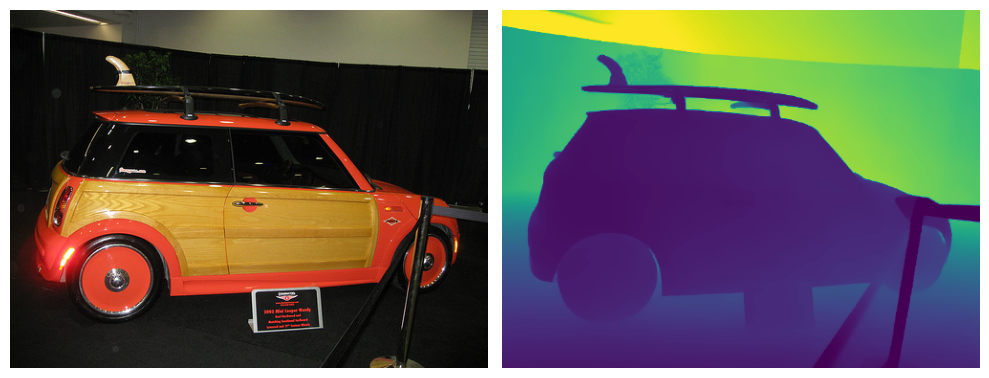
\includegraphics[width=1\linewidth]{./images/Original-vs-Marigold.png}
    \caption{Side-by-side comparison between an original ImageNet RGB image and its estimated depth map using Marigold.}
    \label{fig:imagenet-depth-est-example}
\end{figure}

\subsection{ImageNet 200-class depth}
To further reduce computational overhead while maintaining diversity in object categories, we constructed a 200-class subset of previously mentioned dataset (Imagenet 1k-class depth) by randomly sampling 200 classes from the full 1,000-class set. This subset contains 10,000 images, with 50 images per class. The list of sampled classes can be found in the \href{https://gitlab.com/dariofurlan/vcs-2425/}{Supplementary Material}. This smaller subset is more balanced and allows us to conduct more detailed evaluations by reducing label space complexity while also preserving the large-scale nature of ImageNet.

\subsection{Washington-RGB-D}
The Washington RGB-D Object Dataset \cite{washington-rgbd} is a real-world RGB-D dataset widely used in robotics and object recognition research. It was captured by a Microsoft Kinect sensor and contains 51 categories of common indoor objects (e.g., scissors, cereal boxes, keyboards) with 300 distinct object instances.

The training set includes 207,920 RGB-D frames, and the validation set (which we use in our study) has 41,877 images. Each instance is recorded from three video sequences, with one frame extracted every fifth frame. For each image, the dataset provides aligned RGB, raw depth (in millimeters), segmentation masks, and cropping metadata.

We specifically use the \textit{depthcrop.png} files, which are single-channel, 16-bit depth images. These real depth images were used as-is, with only minor preprocessing. While the dataset was originally intended for object recognition and pose estimation, we repurpose it for our depth-only classification task. 

\subsection{Preprocessing}

Convolutional Neural Networks (CNNs) are typically designed to operate on 3-channel, 8-bit RGB images of fixed dimensions. However, our experiments focus on depth images, which differ significantly in structure and format. Therefore, several preprocessing steps, such as resizing and normalization to standardize input dimensions and pixel value ranges, are necessary to adapt the datasets to the input requirements of standard classification architectures.

% \subsubsection{Depth Estimation for ImageNet}

\subsubsection{Color Mapping Depth Maps for CNNs}
Depth images are single-channel and thus incompatible with CNNs pretrained on RGB data like AlexNet, VGG19, ResNet50 and Inception-v3. To bridge this gap, we convert them into three-channel inputs using perceptually uniform colormaps and a custom stacked encoding. Unlike the commonly used jet (rainbow) colormap, these mappings preserve perceptual ordering and reduce visual artifacts that may impair representation learning \cite{rainbow_harmful}. This process is composed of two main steps:

\begin{itemize}
    \item Normalization: The 16-bit depth values (range: 0-65,535) are scaled down to 8-bit values (range: 0-255) using min-max normalization.
    \item Channel Expansion: We convert the single-channel 8-bit image into a 3-channel image using two main strategies:
    \begin{itemize}
        \item Channel Duplication (Stacking): Simply by replicating the depth channel across all three channels.
        \item Colormap Mapping: We apply perceptually uniform colormaps (Viridis, Plasma, Magma and Grayscale) to produce pseudo-RGB images, allowing us to investigate whether color encoding affects feature extraction as shown in the \autoref{fig:depth-color-mapping-examples}.
    \end{itemize}
\end{itemize}

\begin{figure}[h]
    \centering
    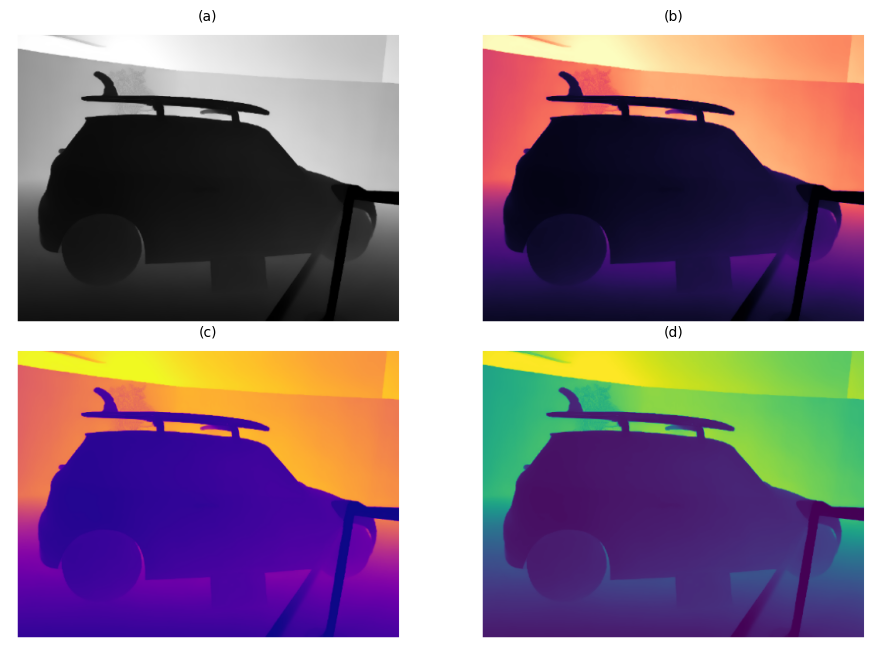
\includegraphics[width=1\linewidth]{./images/stacked-plasma-virdis-and-magma.png}
    \caption{Examples of 8-bit 3-channel depth images obtained through different preprocessing methods: (a) stacked and grayscale, (b) Magma, (c) Plasma, and (d) Viridis colormaps. \\ \textit{Note that grayscale and stacked images are visually similar, as they both represent depth information without color encoding.}}
    \label{fig:depth-color-mapping-examples}
\end{figure}

\subsubsection{Preprocessing the Washington RGB-D Dataset}
The Washington RGB-D dataset already includes 16-bit depth maps captured via Kinect. We applied the same post-processing steps used for ImageNet: 16-bit depth values to 8-bit normalization, and conversion to 3-channel format via channel duplication and colormap mapping. This ensures consistency in input structure across both synthetic and real-world depth data.

\section{Methodology}

We investigate whether standard convolutional neural networks (CNNs) can effectively classify objects using depth-only inputs, a question motivated by the need for privacy-preserving computer vision.

\subsection{Architectures}

To assess performance across different model families and depths, we evaluate four well-known CNN architectures, originally developed for RGB image classification:

\begin{itemize}
    \item \textbf{AlexNet}: a relatively shallow model with fewer parameters, representing the early generation of deep learning-based classifiers \cite{alexnet}.
    \item \textbf{VGG19}: a deeper model with a straightforward design based on stacked $3 \times 3$ convolutions \cite{vgg19}.
    \item \textbf{ResNet50}: a residual network with 50 layers and identity shortcut connections, allowing for effective training of deeper models \cite{resnet50}.
    \item \textbf{Inception-v3}: an architecture that uses parallel convolutional paths and factorized filters to balance efficiency and performance \cite{inceptionv3}.
\end{itemize}

These models were chosen to cover a range of architectural complexity and to observe whether trends in RGB image classification carry over to depth-only data.

\subsection{Training Regimes}

Each model is evaluated under three distinct training configurations:
\begin{itemize}
    \item \textbf{Baseline}: The model is evaluated using its original pre-trained weights, without any adaptation to the depth modality.
    \item \textbf{Partial Fine-tuning}: Only the final classification layers are made trainable, allowing limited adaptation to the depth input.
    \item \textbf{Complete Fine-tuning}: All parameters are made trainable, enabling full adaptation of the network to the new data modality.
\end{itemize}

\subsection{Evaluation Protocol}

Not all training regimes are applied to all datasets due to dataset-specific constraints. Baseline evaluation is performed only on the \textit{ImageNet 1k-class depth} dataset, where pre-trained models can be meaningfully assessed without retraining. Both partial and complete fine-tuning are applied where sufficient training data is available (\textit{ImageNet 1k-class and 200-class depth}), while the smaller \textit{Washington RGB-D} dataset is used only with partial fine-tuning to avoid overfitting.

We use classification \textbf{accuracy} as our main evaluation metric, and report both \textbf{Top-1} accuracy (the correct label is the highest-ranked prediction) and \textbf{Top-5} accuracy (the correct label is among the five highest-ranked predictions). For baseline evaluations, the entire dataset is used for testing. In fine-tuning settings, we adopt a standard 80/20 split for training and validation.
\section{Experiments}
In this section, we present three experiments conducted to evaluate the performance of pretrained models on depth images. First, we establish a baseline by comparing model accuracy across different colormaps applied to the depth images. Second, we explore the impact of fine-tuning on model performance using the stacked colormap representation. Finally, we assess the models on subsets of ImageNet and the Washington RGB-D dataset to understand their behavior on tasks with reduced label spaces and lower complexity.

\subsection{ImageNet 1k-class Depth}
We initiated our experiments by evaluating the performance of the models ``as-is'', without any fine-tuning applied to the depth images.

The models employed in this study (AlexNet, VGG19, InceptionV3, ResNet50) were conveniently pretrained on the same 1,000 classes as our dataset. This alignment was achieved by carefully curating the dataset, thereby obviating the need to fine-tune the final layer of the classifier, as it already produced the correct labels.

To establish a baseline and investigate whether the models exhibited varying performance under different colormaps of the depth images, we experimented with a stacked approach, grayscale, viridis, plasma and magma colormaps as shown in \autoref{fig:model_acc_by_colormap} and summarized in \autoref{tab:baseline_accuracy}.

\begin{figure}[h]
    \centering
    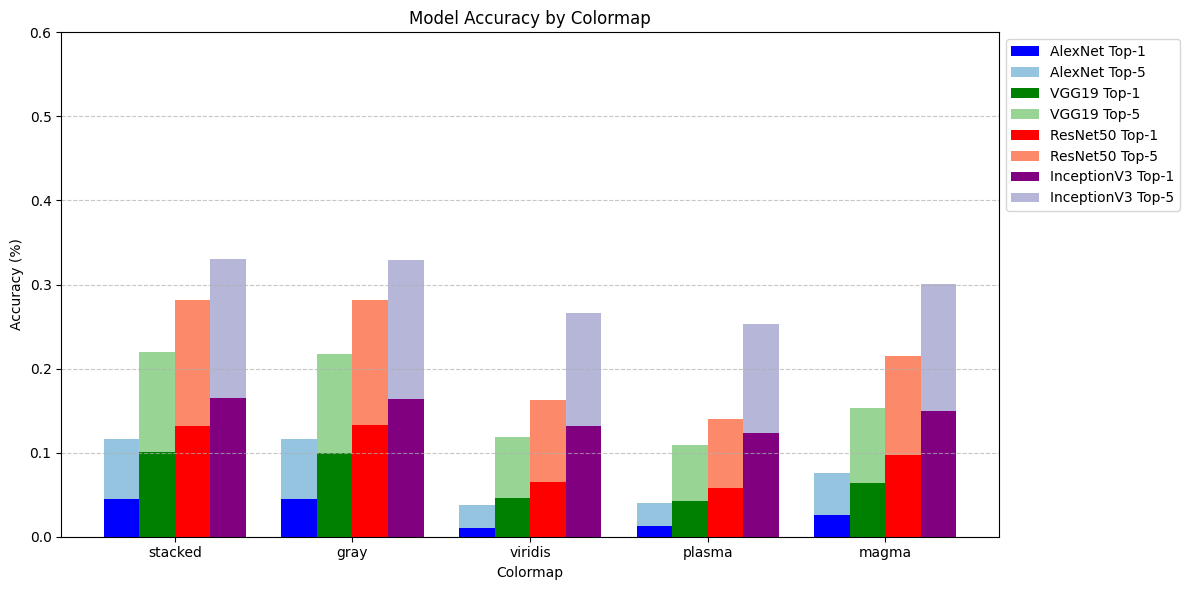
\includegraphics[width=1\linewidth]{./images/model_acc_by_colormap.png}
    \caption{Baseline accuracy comparison across colormaps for ImageNet 1k-class depth.}
    \label{fig:model_acc_by_colormap}
\end{figure}

\begin{table*}[htbp]
    \centering
    \begin{tabular}{|l|c|c|c|c|c|c|c|c|c|c|c|c|}
        \hline
        \multirow{2}{*}{Model} & \multicolumn{2}{|c|}{Stacked} & \multicolumn{2}{|c|}{Grayscale} & \multicolumn{2}{|c|}{Viridis} & \multicolumn{2}{|c|}{Plasma} & \multicolumn{2}{|c|}{Magma} \\
        \cline{2-11}
         & Top-1 & Top-5 & Top-1 & Top-5 & Top-1 & Top-5 & Top-1 & Top-5 & Top-1 & Top-5 \\
        \hline
        AlexNet & \textbf{04.53} & \textbf{11.63} & 04.50 & 11.62 & 01.04 & 03.83 & 01.24 & 03.98 & 02.54 & 07.59 \\
        \hline
        VGG19 & \textbf{10.04} & \textbf{22.00} & 09.97 & 21.79 & 04.64 & 11.87 & 04.29 & 10.95 & 06.45 & 15.31 \\
        \hline
        ResNet50 & 13.18 & \textbf{28.16} & \textbf{13.27} & 28.16 & 06.56 & 16.23 & 05.83 & 14.00 & 09.71 & 21.44 \\
        \hline
        InceptionV3 & \textbf{16.48} & \textbf{33.05} & 16.40 & 32.94 & 13.16 & 26.66 & 12.36 & 25.34 & 15.01 & 30.07 \\
        \hline
    \end{tabular}
    \caption{Baseline accuracy comparison across colormaps for ImageNet 1k-class depth.}
    \label{tab:baseline_accuracy}
\end{table*}

\begin{table*}[htbp]
    \centering
    \begin{tabular}{|l|cc|cc|cc|}
        \hline
        \multicolumn{1}{|c|}{\multirow{2}{*}{Model}} & \multicolumn{2}{c|}{Baseline} & \multicolumn{2}{c|}{Partial Fine-Tuning} & \multicolumn{2}{c|}{Fine-Tuning}                                 \\ \cline{2-7} 
        \multicolumn{1}{|c|}{}                       & \multicolumn{1}{c|}{Top-1}  & Top-5 & \multicolumn{1}{c|}{Top-1}    & Top-5    & \multicolumn{1}{c|}{Top-1}                & Top-5                \\ \hline
        AlexNet                                      & \multicolumn{1}{c|}{04.53}  & 11.63 & \multicolumn{1}{c|}{18.05}    & 36.41    & \multicolumn{1}{c|}{\textbf{23.62}}       & \textbf{45.76}       \\ \hline
        VGG19                                        & \multicolumn{1}{c|}{10.04}  & 22.00 & \multicolumn{1}{c|}{25.40}    & 48.18    & \multicolumn{1}{c|}{\textbf{34.20}}       & \textbf{60.96}       \\ \hline
        ResNet50                                     & \multicolumn{1}{c|}{13.18}  & 28.16 & \multicolumn{1}{c|}{32.36}    & 57.87    & \multicolumn{1}{c|}{\textbf{44.95}}       & \textbf{71.90}       \\ \hline
        InceptionV3                                  & \multicolumn{1}{c|}{16.48}  & 33.05 & \multicolumn{1}{c|}{22.31}    & 44.57    & \multicolumn{1}{c|}{\underline{\textbf{48.53}}} & \underline{\textbf{74.53}} \\ \hline
    \end{tabular}
    \caption{Fine-tuning accuracy comparison for ImageNet 1k-class depth.}
    \label{tab:finetuning_accuracy}
\end{table*}

This experiment demonstrated that the grayscale approach yielded results most familiar to the models. Furthermore, we established that a straightforward approach, such as duplicating the original single-channel depth image to the three channels required by these models, is as robust as applying a colormap function to the grayscale image.

Further experimentation involving fine-tuning these models resulted in a significant increase in accuracy. Given the strong performance of the "stacked" colormap, we focused on this approach for fine-tuning and excluded other colormaps from further analysis.

The partial fine-tuning procedure involved freezing all model parameters except for a small subset of layers that were specifically selected for training. In the case of \textbf{AlexNet}, only the final \texttt{classifier} layer was unfrozen and trained. For \textbf{VGG19}, we applied the same strategy, unfreezing only the \texttt{classifier} module. In the case of \textbf{ResNet50}, we unfroze both the last residual block (\texttt{layer 4}) and the final fully connected layer (\texttt{layer 5}). Finally, for \textbf{InceptionV3}, the fine-tuning was performed by unfreezing the last inception block (\texttt{Mixed\_7c}), the auxiliary classifier (\texttt{AuxLogits}), and the final fully connected layer (layer 5).

The complete fine-tuning procedure involved unfreezing all model parameters, allowing the models to adapt fully to the depth images. This approach was computationally more expensive but yielded higher accuracy.

As reported in \autoref{tab:finetuning_accuracy}, both partial and full fine-tuning substantially improved model performance on depth images. The stacked colormap representation proved effective, with InceptionV3 achieving the highest Top-1 accuracy (48.53\%) and Top-5 accuracy (74.53\%). These results suggest that models originally developed for RGB image classification retain their relative performance ranking when applied to depth data. For instance, architectures that achieve higher accuracy on RGB tasks (e.g., InceptionV3 vs. AlexNet) also perform better on depth images, indicating that the improvements are architecture-driven rather than modality-specific.

While both fine-tuning strategies enhanced the models' ability to interpret depth images, the limited number of examples per class in our dataset constrained the overall performance. Nonetheless, the improvements observed with complete fine-tuning are notable: on average, we recorded a nearly \textbf{3x} increase in accuracy compared to the baseline (computed as the mean ratio between full fine-tuning and baseline results for Top-1 and Top-5 across all models). 
% This supports further exploration in this direction.

\subsection{ImageNet Subset (200 Classes)}

As shown in Table 3, full fine-tuning consistently outperforms partial fine-tuning across all models on the 200-class subset. InceptionV3 achieves the highest Top-1 accuracy (47.95\%, 72.80\% ), while ResNet50 leads in Top-5 accuracy (47.75\%, 73.20\%). The relative performance ranking of the models aligns with the results from the 1000-class subset, indicating stable model behavior despite the smaller dataset size. Both fine-tuning approaches improve performance; however, deeper networks benefit more substantially from full fine-tuning, highlighting the importance of end-to-end adaptation when working with limited data.

\begin{table*}[htbp]
    \centering
    \begin{minipage}[t]{0.48\textwidth}
        \centering
        \begin{tabular}{|l|c|c|c|c|}
            \hline
            \multirow{2}{*}{Model} & \multicolumn{2}{|c|}{Partial FT} & \multicolumn{2}{|c|}{Complete FT} \\ \cline{2-5}
             & Top-1 & Top-5 & Top-1 & Top-5 \\
            \hline
            AlexNet & 26.25 & \textbf{52.90} & \textbf{26.40} & 51.25 \\
            \hline
            VGG19 & 32.50 & 59.95 & \textbf{36.70} & \textbf{65.25} \\
            \hline
            ResNet50 & 44.30 & 71.15 & \textbf{47.75} & \textbf{73.20} \\
            \hline
            InceptionV3 & 38.70 & 64.15 & \textbf{47.95} & \textbf{72.80} \\
            \hline
        \end{tabular}
        \caption{Accuracy on 200-class ImageNet subset.}
        \label{tab:imagenet_subset_accuracy}
    \end{minipage}
    \hfill
    \begin{minipage}[t]{0.48\textwidth}
        \centering
        \begin{tabular}{|l|c|c|}
            \hline
            Model & Top-1 & Top-5 \\
            \hline
            AlexNet & 87.51 & 98.79 \\
            \hline
            VGG19 & 92.23 & 99.61 \\
            \hline
            ResNet50 & 88.48 & 99.31 \\
            \hline
            InceptionV3 & 89.45 & 99.08 \\
            \hline
        \end{tabular}
        \caption{Partial fine-tuning accuracy on Washington RGB-D.}
        \label{tab:washington_rgbd_accuracy}
    \end{minipage}
\end{table*}

\subsection{Washington RGB-D Dataset}
Following the same approach we used again the stacked colormap representation for the Washington RGB-D dataset. In contrast, the Washington RGB-D dataset comprises only 51 classes, with an average of 821 images per class, unlike ImageNet, which has only 50, representing a significantly lower task complexity and substantially larger training data. 

As reported in Table 4, all models achieved near 90\% Top-1 accuracy, with VGG19 reaching up to 92.23\%. These results were obtained using partial fine-tuning alone. Given this high baseline, we opted not to undertake complete fine-tuning, concluding that the incremental improvements would not justify the higher computational expense. 

Overall, for sufficiently large datasets, transfer learning tends to be highly effective, eliminating the need for complete fine-tuning.

\section{Conclusion and Future Work}

This work has demonstrated that depth-only images can achieve competitive performance in image classification tasks using standard convolutional neural networks (CNNs) pretrained on RGB data. Our results indicate that, even without fine-grained texture or color, depth information alone can provide sufficient structure for effective classification across both synthetic and real-world datasets.

\begin{itemize}
    \item \textbf{High accuracy on real-world data:} On the Washington RGB-D dataset, models such as VGG19 surpassed 92\% Top-1 accuracy, confirming the viability of depth-only inputs in practical, privacy-sensitive environments.
    
    \item \textbf{Use of existing architectures:} By applying minimal preprocessing—normalization, channel stacking, and colormap mapping—we successfully adapted standard architectures (e.g., ResNet50, InceptionV3, VGG19) to operate on depth images without requiring modifications to the model structure.
    
    \item \textbf{Effectiveness of fine-tuning:} Fine-tuning, even when limited to later layers, consistently improved classification performance, especially in complex scenarios such as the full 1,000-class ImageNet subset, where baseline accuracies more than doubled after training.
    
    \item \textbf{Privacy-aware vision:} Depth images inherently lack identifying features such as facial detail or clothing patterns, making them particularly well-suited for computer vision applications in domains requiring privacy, such as healthcare, education, and public surveillance.
\end{itemize}

\subsection{Future Work}
A key limitation of this study is the limited number of depth samples per class, due to the scarcity of large-scale depth-only image classification datasets. To address this, we plan to scale our experiments to the full ImageNet dataset with estimated depth maps, enabling evaluation in a higher-data regime and testing the scalability of our approach.

Additionally, adapting single-channel depth maps to standard three-channel CNN inputs poses a challenge. To this end, future work will explore learned depth encodings via lightweight autoencoder networks, as demonstrated in \cite{carlucci2018de2codeepdepth}, which proposes a deep learning approach to transform depth images into RGB format.

Moreover, we intend to extend our exploration beyond classification to the task of \textit{semantic segmentation}. While high-quality depth-based datasets for image classification remain scarce, numerous segmentation datasets include depth information. This shift will enable a broader and more realistic evaluation of depth-only models in structured prediction tasks, and may provide further evidence for the suitability of depth data in privacy-sensitive vision applications.

Ultimately, this line of research seeks to develop practical and privacy-conscious computer vision systems that do not compromise on performance, while avoiding reliance on RGB data.

{\small
\bibliographystyle{ieee_fullname}
\bibliography{egbib}
}

\end{document}
